\documentclass[11pt,a4paper]{article}

% ── Packages ─────────────────────────────────────────────────────────────────
\usepackage[margin=1in]{geometry}
\usepackage{amsmath,amssymb}
\usepackage{graphicx}
\usepackage{booktabs}
\usepackage{hyperref}
\usepackage{caption}
\usepackage{subcaption}
\usepackage{float}
\usepackage[numbers,sort&compress]{natbib}
\usepackage{enumitem}
\usepackage{xcolor}
\usepackage{microtype}
\usepackage{parskip}

% ── Metadata ─────────────────────────────────────────────────────────────────
\title{\textbf{COMP0051 Algorithmic Trading Coursework}\\[4pt]
       \large Walk-Forward Trend-Following and BTC-Dominance Mean-Reversion\\
       in Cryptocurrency Markets}
\author{Peter Prendergast\\
        University College London\\
        \texttt{peterdunmain@outlook.com}}
\date{\today}

% ── Custom commands ──────────────────────────────────────────────────────────
\newcommand{\usdt}{\text{USDT}}
\newcommand{\Cov}{\operatorname{Cov}}
\newcommand{\Var}{\operatorname{Var}}
\newcommand{\sgn}{\operatorname{sgn}}
\newcommand{\abs}[1]{\lvert #1 \rvert}

\begin{document}
\maketitle
\thispagestyle{empty}

% =============================================================================
% SECTION 1 — Data Download and Visualisation [10 points]
% =============================================================================
\section{Data Download and Visualisation}
\label{sec:data}

\subsection{Data Acquisition}

We source daily OHLCV (open, high, low, close, volume) bars for four major cryptocurrency pairs---BTC/USDT, ETH/USDT, BNB/USDT, and ADA/USDT---from the Binance exchange via the \texttt{ccxt} unified API, covering the period from 1~January~2020 to 20~March~2026.  The resulting dataset comprises 2{,}271 daily observations per asset.  We select daily frequency as a compromise between capturing medium-term momentum dynamics and maintaining manageable data volumes; this granularity aligns with the findings of Liu and Tsyvinski~\cite{liu2021}, who document significant time-series momentum effects in cryptocurrency markets at horizons ranging from one day to several weeks.  The four assets were chosen to span a range of market capitalisations and liquidity profiles: BTC and ETH represent the two most liquid cryptocurrencies, while BNB and ADA provide exposure to mid-cap altcoins with meaningfully different volatility characteristics.  All data are persisted in Apache Parquet format via \texttt{pyarrow} for efficient columnar storage and fast I/O during iterative backtesting.

Strategy~2 draws on a broader universe of 11 Binance spot pairs (BTC, ETH, BNB, SOL, XRP, ADA, AVAX, DOT, LINK, LTC, MATIC) to construct a diversified altcoin basket and a BTC-dominance signal.  These additional assets are fetched on the same daily grid and aligned to the Strategy~1 calendar via inner join.

\subsection{Data Cleaning and Outlier Treatment}

The raw OHLCV data undergo a multi-stage cleaning pipeline.  First, duplicate timestamps are removed by retaining only the earliest observation at each index.  All price and volume columns are coerced to numeric types, and rows failing basic validity constraints---such as non-positive prices, negative volumes, or violations of the OHLC ordering rule ($h_t \geq \max(o_t, c_t)$ and $l_t \leq \min(o_t, c_t)$)---are dropped.  We then compute simple returns $r_t = (c_t - c_{t-1})/c_{t-1}$ and flag statistical outliers using a rolling z-score method: for each bar, we calculate $z_t = (r_t - \bar{r}_t^{(24)}) / \hat{\sigma}_t^{(24)}$, where $\bar{r}_t^{(24)}$ and $\hat{\sigma}_t^{(24)}$ denote the rolling mean and standard deviation over a 24-bar window (with a minimum of 8 observations), respectively.  Observations satisfying $\abs{z_t} > 5$ are flagged as outliers.  Outliers are flagged but not removed, preserving the integrity of the time series for downstream rolling-window calculations.

A quality audit is performed at both the raw and cleaned stages for each asset, recording the number of rows, duplicate timestamps, missing bars (relative to an ideal daily grid), null values, and flagged outliers.  The audit confirms zero structural issues across all four assets: no duplicates, no missing bars, and no null rows in either the raw or cleaned stages.

\subsection{Risk-Free Rate and Excess Returns}

We download the daily Effective Federal Funds Rate (DFF) from the Federal Reserve Economic Data (FRED) database.  The annualised rate is converted to a daily return via $(1 + \text{DFF}/100)^{1/365} - 1$ and forward-filled to cover weekends and holidays.  Excess simple returns are formed as:
\begin{equation}
  r^e_t = \frac{p_t - p_{t-1}}{p_{t-1}} - r^f_{t},
  \label{eq:excess-return}
\end{equation}
where $r^f_{t}$ is the per-day risk-free rate.

At daily frequency, the risk-free component remains economically small relative to cryptocurrency return volatility.  We therefore use simple returns for signal construction throughout and treat excess returns as an available robustness check (controlled by the \texttt{BACKTEST\_USE\_EXCESS} flag in our configuration).  This decision is consistent with the common practice in cryptocurrency research of ignoring $r^f$ when the holding period is sufficiently short~\cite{liu2021}.

\begin{figure}[H]
  \centering
  % 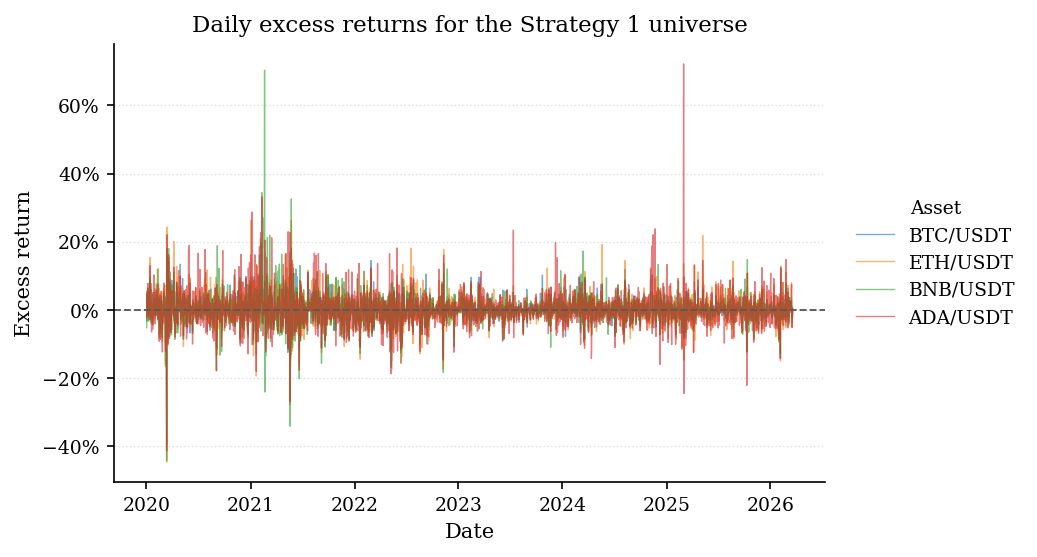
\includegraphics[width=\textwidth]{output/daily_excess_returns.png}
  \caption{Daily excess return time series for BTC/USDT, ETH/USDT, BNB/USDT, and ADA/USDT (January 2020--March 2026).}
  \label{fig:return-ts}
\end{figure}


% =============================================================================
% SECTION 2 — Strategy [40 points]
% =============================================================================
\section{Strategy Development}
\label{sec:strategy}

We develop two complementary trading strategies---a time-series trend-following strategy and a BTC-dominance mean-reversion strategy---subject to the gross exposure constraint $\sum_i \abs{\theta^i_t} \leq \$100{,}000$ at all times, with initial capital $V_0 = \$10{,}000$.  This implies a maximum permissible leverage of $10\times$.  Both strategies are implemented within an event-driven backtesting engine that processes each bar sequentially, maintaining realistic path-dependent state including equity tracking, leverage monitoring, and an insolvency circuit-breaker that liquidates all positions if equity reaches zero.

% -----------------------------------------------------------------------------
\subsection{Strategy 1: Trend Following}
\label{sec:trend}

\subsubsection{Economic Rationale}

Time-series momentum---the tendency for assets that have recently appreciated to continue appreciating, and vice versa---has been documented across a wide range of asset classes by Moskowitz, Ooi, and Pedersen~\cite{moskowitz2012} and subsequently in cryptocurrency markets by Liu and Tsyvinski~\cite{liu2021}.  The economic rationale rests on a combination of behavioural underreaction to new information and the self-reinforcing dynamics of trend-following capital flows.  Our strategy exploits this effect by measuring the distance of the current price from a trailing moving average, normalised by recent volatility, and taking directional positions proportional to the strength and sign of this signal.

\subsubsection{Signal Construction}

For each asset $i$ at time $t$ we compute a volatility-normalised trend signal in two stages.  First, the raw trend measure captures the fractional deviation of the current close price $p_{i,t}$ from its $w$-bar simple moving average:
\begin{equation}
  \text{trend\_raw}_{i,t} = \frac{p_{i,t}}{\text{MA}_{i,t}(w)} - 1,
  \label{eq:trend-raw}
\end{equation}
where $\text{MA}_{i,t}(w) = \frac{1}{w}\sum_{k=0}^{w-1} p_{i,t-k}$.  This raw signal is then standardised by dividing by the rolling standard deviation of simple returns over a $w_{\text{vol}}$-bar window:
\begin{equation}
  z_{i,t} = \frac{\text{trend\_raw}_{i,t}}{\sigma_{i,t}(w_{\text{vol}})},
  \label{eq:trend-z}
\end{equation}
where $\sigma_{i,t}(w_{\text{vol}}) = \text{std}(r_{i,t-w_{\text{vol}}+1}, \ldots, r_{i,t})$ with $\text{ddof}=0$.  The z-score is clipped at $\pm 5$ to limit the influence of extreme readings.  The position direction is then determined by a dead-zone threshold $\delta$: if $z_{i,t} > \delta$, the asset receives a long signal ($+1$); if $z_{i,t} < -\delta$, a short signal ($-1$); otherwise the asset is flat ($0$).  This discrete activation prevents noisy oscillations near zero from generating spurious round-trips.

Crucially, the z-score is used \emph{only} for dead-zone activation, not for dollar sizing.  The subsequent position-sizing step uses the raw trend signal divided by rolling volatility as a single, unified risk-adjustment.

\subsubsection{Position Sizing via Simplified Mean-Variance Optimisation}
\label{sec:mvo}

The brief requires the use of mean-variance optimisation (MVO) or a cost-aware method for setting exposures $\theta_t$ at each rebalancing point.  We employ a volatility-inverse weighting scheme that can be derived as the closed-form solution to a simplified MVO problem.

Consider the standard Markowitz objective of maximising expected return for a given level of risk, subject to a gross exposure constraint.  Under two simplifying assumptions---equal expected excess returns across all active assets ($\mu_i = \mu$ for all $i$ with $d_{i,t} \neq 0$) and a diagonal covariance matrix ($\Sigma = \text{diag}(\sigma_1^2, \ldots, \sigma_k^2)$, i.e.\ zero cross-asset correlation)---the optimal weight vector $w^*$ that minimises portfolio variance for a given expected return is proportional to $\Sigma^{-1}_{ii} = 1/\sigma_i^2$.

The sizing pipeline proceeds as follows.  On active bars (where $\abs{z_{i,t}} > \delta$), the raw weight is $w^{\text{raw}}_{i,t} = \text{trend\_raw}_{i,t}$; on inactive bars it is zero.  A single volatility-adjustment step produces the risk weight:
\begin{equation}
  w^{\text{risk}}_{i,t} = \frac{w^{\text{raw}}_{i,t}}{\sigma_{i,t}(w_{\text{vol}})}.
  \label{eq:risk-weight}
\end{equation}
These are then $L_1$-normalised:
\begin{equation}
  \tilde{w}_{i,t} = \frac{w^{\text{risk}}_{i,t}}{\sum_j \abs{w^{\text{risk}}_{j,t}}},
  \label{eq:vol-inv-weights}
\end{equation}
such that $\sum_j \abs{\tilde{w}_{j,t}} = 1$ on active bars.  Dollar exposures are then:
\begin{equation}
  \theta_{i,t} = \tilde{w}_{i,t} \times G,
  \label{eq:theta}
\end{equation}
where $G = \$100{,}000$ is the gross notional cap.  With $V_0 = \$10{,}000$, this permits up to $10\times$ leverage.

The diagonal covariance assumption is a deliberate simplification; in practice, cryptocurrency returns exhibit significant positive cross-asset correlation, particularly during market stress events.  However, the diagonal approximation avoids the well-known instability of full covariance matrix estimation in small cross-sections ($k = 4$ assets) and at daily frequency, where noise in off-diagonal elements can lead to extreme and poorly conditioned weight vectors.

\subsubsection{Rebalancing}

Positions are rebalanced at a configurable frequency of every $n$ days; between rebalancing events, positions are carried forward and grow or shrink with the underlying asset returns: $\theta^{\text{carried}}_{i,t} = \theta^{\text{exec}}_{i,t-1} \times (1 + r_{i,t})$.  This carry-forward mechanism is critical for realistic backtesting, as it captures the path-dependent drift in exposure that occurs between discrete rebalancing points.

\subsubsection{Walk-Forward Parameter Selection}
\label{sec:trend-wf}

All strategy parameters are selected via a walk-forward validation procedure to prevent look-ahead bias.  The full dataset is divided into a development sample and a final untouched test window comprising the last 126 daily bars (approximately 6~months, from 15~November~2025 to 20~March~2026).  A historical holdout of $22.5\%$ is additionally noted but treated as contaminated because multiple alternative configurations were inspected against it during development.

Within the development sample, we construct expanding-window walk-forward folds: the initial training window spans 600 daily bars (approximately 2.4~years), and the validation window covers 100 bars (approximately 4~months), with non-overlapping validation segments advancing by 100 bars per fold.  This yields 15 walk-forward folds spanning diverse market regimes.

For the trend strategy, we search over the following parameter grid: moving average window $w \in \{80, 120, 160\}$ days, volatility window $w_{\text{vol}} \in \{25, 40\}$ days, dead-zone threshold $\delta \in \{0.75, 1.0, 1.25\}$, and rebalancing frequency $n \in \{5, 10\}$ days.  The signal clip is fixed at $\pm 5$ and the gross cap at $\$100{,}000$.

Each candidate parameter combination is evaluated by running the full backtest on the development sample and computing the Sharpe ratio over each validation fold.  The selection criterion is the stability-penalised mean validation Sharpe:
\begin{equation}
  \text{score} = \overline{S}_{\text{val}} - \lambda \cdot \text{std}(S_{\text{val}}),
  \label{eq:wf-score}
\end{equation}
where $\overline{S}_{\text{val}}$ is the mean Sharpe across folds, $\text{std}(S_{\text{val}})$ is the cross-fold standard deviation, and $\lambda = 0.1$ is the stability penalty.  A candidate is considered valid only if: (i) mean validation Sharpe is positive, (ii) at least $55\%$ of folds have positive Sharpe, and (iii) mean validation turnover does not exceed $\$4{,}000$.  Among valid candidates, the highest-scoring configuration is selected; when multiple candidates fall within $5\%$ of the best score, ties are broken by lower turnover, then higher mean return, then lower absolute maximum drawdown.  If no candidate passes the hard filters, the default anchor configuration ($w = 120$, $w_{\text{vol}} = 40$, $\delta = 1.25$, $n = 10$) is used as a fallback.

The walk-forward procedure selects $w = 120$ days, $w_{\text{vol}} = 40$ days, $\delta = 1.25$, and $n = 10$ days, with a mean validation Sharpe of $0.39$ and a walk-forward score of $0.26$.

\begin{figure}[H]
  \centering
  % 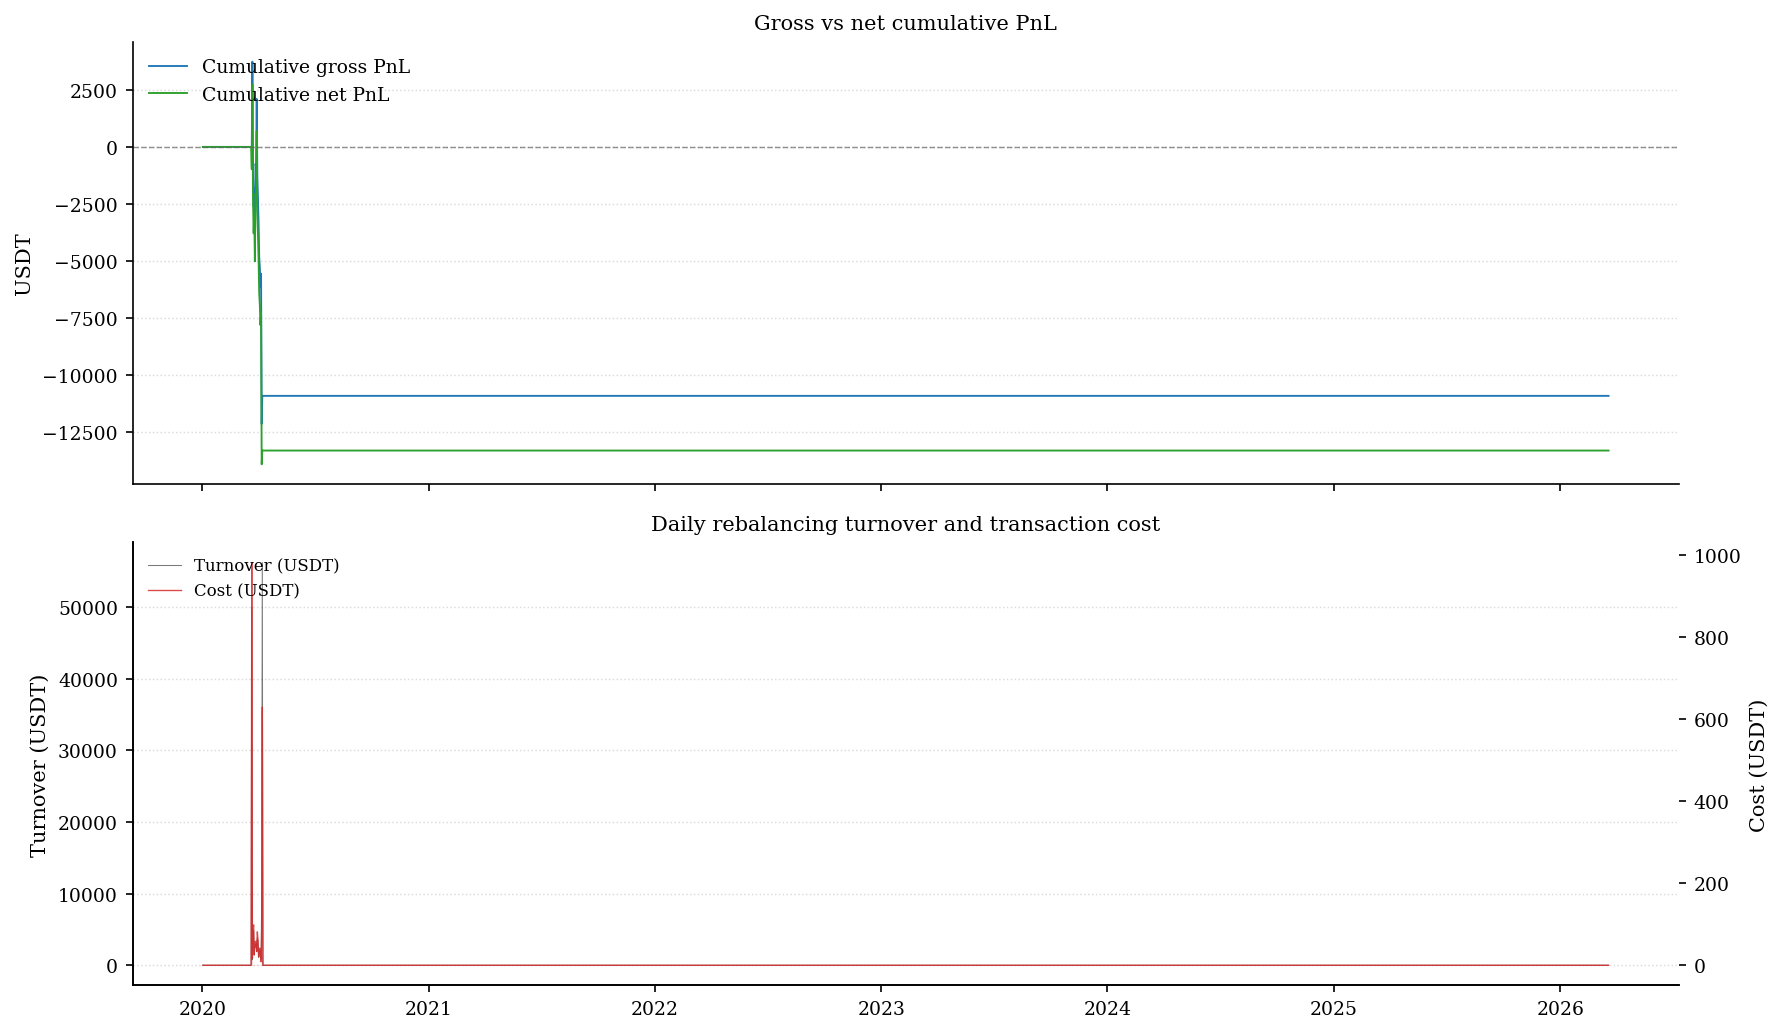
\includegraphics[width=\textwidth]{output/net_vs_gross_cost_turnover.png}
  \caption{Strategy~1 (trend) gross vs.\ net cumulative PnL and daily turnover/cost breakdown.}
  \label{fig:trend-equity}
\end{figure}

\begin{figure}[H]
  \centering
  % 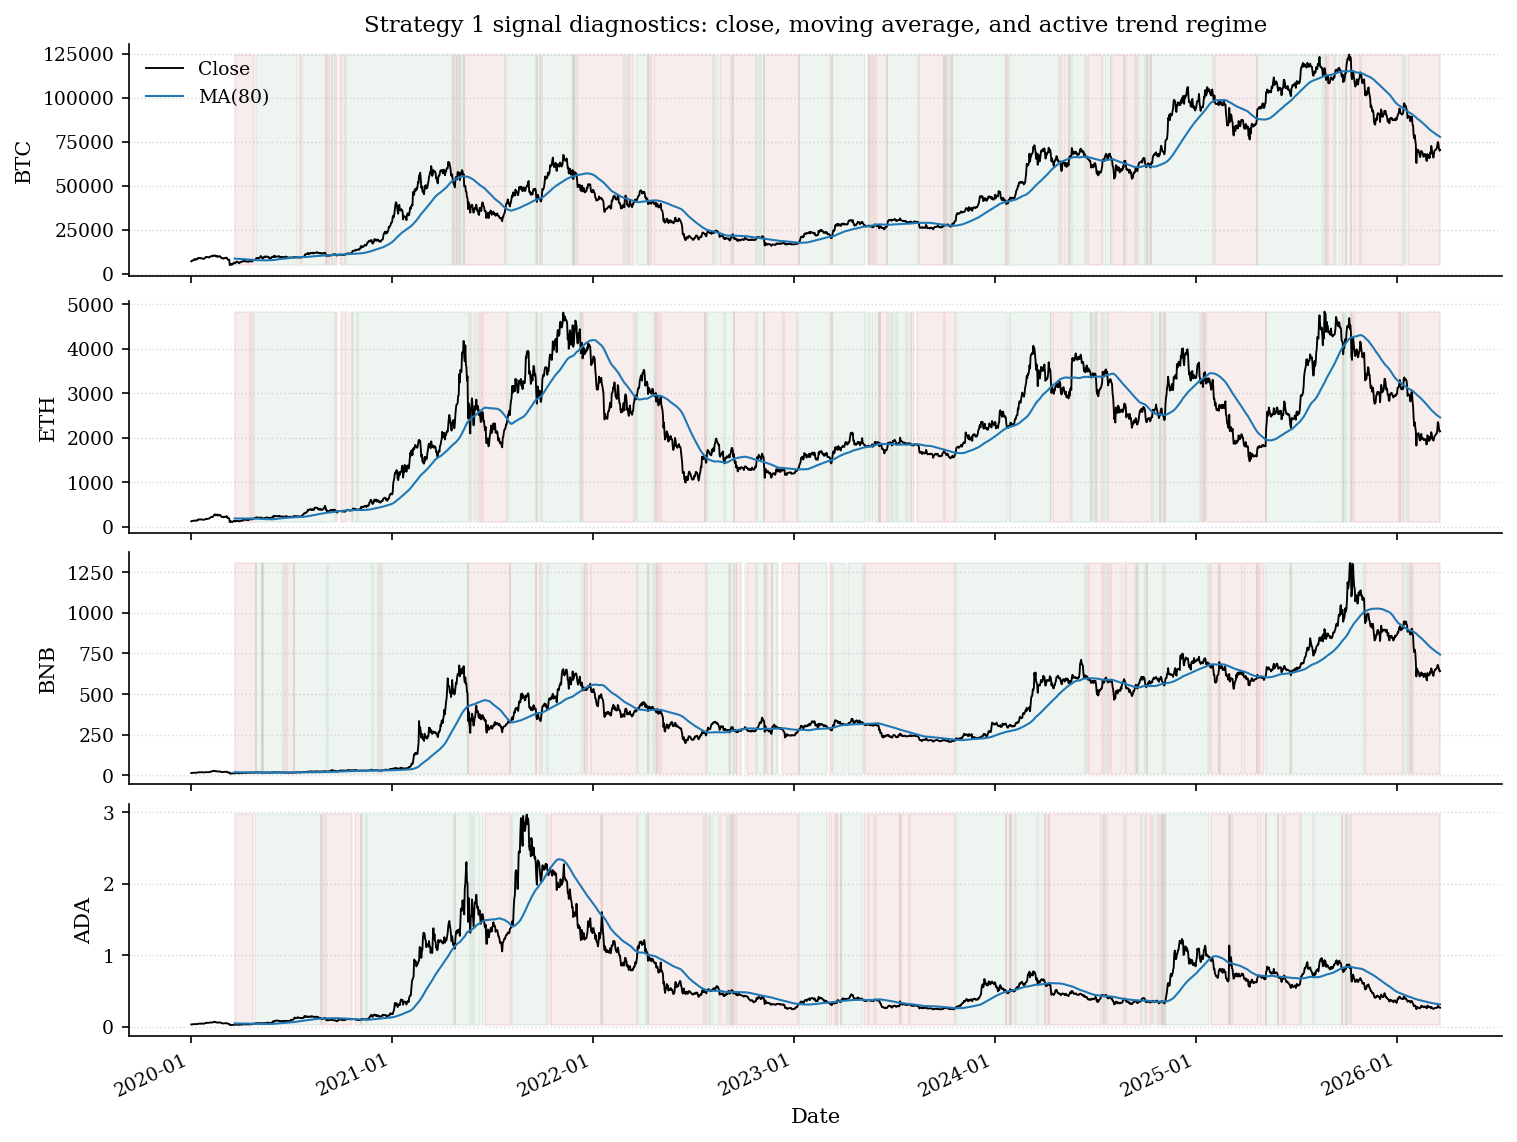
\includegraphics[width=\textwidth]{output/trend_signals_vs_price.png}
  \caption{Trend signal regimes (long/flat/short) for each asset over the full sample period.  Green shading denotes long positions, red denotes short positions, and white denotes flat (no exposure).}
  \label{fig:trend-regimes}
\end{figure}

% -----------------------------------------------------------------------------
\subsection{Strategy 2: BTC-Dominance Mean Reversion}
\label{sec:domrsi}

\subsubsection{Economic Rationale}

When BTC dominance spikes---as measured by BTC's share of aggregate notional trading volume across the broader cryptocurrency universe---capital has typically rotated out of altcoins and into BTC.  This is often driven by fear or uncertainty: investors de-risk by consolidating into the most liquid and perceived-safest crypto asset, leaving the altcoin basket temporarily oversold relative to its own recent history.  A mean-reversion strategy buys the equal-weight altcoin basket on these spikes, expecting risk appetite to recover and capital to rotate back into alts once the panic subsides.

This approach is economically distinct from the Engle--Granger cointegration-based pairs trading strategy commonly employed in the literature~\cite{engle1987}.  Rather than relying on the stationarity of a specific price spread between two assets, the dominance-RSI strategy exploits a cross-sectional rotation effect that operates at the level of the entire market's risk-on/risk-off dynamics.

\subsubsection{Signal Construction}

The signal is built from BTC's notional dominance ratio $D_t = \text{notional}^{\text{BTC}}_t / \sum_{j} \text{notional}^j_t$, where notional is defined as close price times volume for each of the 11 assets in the Strategy~2 universe.  Two indicators are computed from this dominance series.

First, the 10-day z-score of daily dominance changes captures the standardised speed of dominance shifts:
\begin{equation}
  z^{\text{dom}}_t = \frac{\Delta D_t - \overline{\Delta D}_t^{(10)}}{\hat{\sigma}^{(10)}_{\Delta D,t}}.
  \label{eq:dom-zscore}
\end{equation}
Second, a 3-day rate-of-change (ROC) of dominance $\text{ROC}_t = D_t - D_{t-3}$ serves as a speed filter to ensure only fast structural shifts trigger entry, filtering out slow secular drifts.

Entry is triggered when both conditions are met simultaneously: (i) the dominance z-score exceeds its rolling 252-day 75th percentile, and (ii) the dominance ROC exceeds its rolling 252-day 85th percentile.  These adaptive thresholds ensure the strategy recalibrates to the prevailing volatility regime rather than relying on fixed levels.

A crash filter suppresses entry (and forces exit) when BTC's 30-day trailing return falls below $-20\%$, distinguishing between healthy rotation (BTC gains while alts underperform, which is tradeable) and broad sell-offs (everything falls, but alts fall harder, where there is no mean-reversion thesis).

Positions are exited when the dominance z-score drops back to zero (mean reversion achieved), or after a maximum holding period of 5 days, whichever comes first.

\subsubsection{Basket Construction}

When in position, the strategy allocates across the 10 altcoins (excluding BTC) using a volatility-weighted underperformance-tilted basket:
\begin{equation}
  w^{\text{raw}}_{i,t} = \max\bigl(-r^{\text{rel}}_{i,t}(3),\; 0\bigr) \times \frac{1}{\sigma_{i,t}(20)},
  \label{eq:basket-weight}
\end{equation}
where $r^{\text{rel}}_{i,t}(3) = r_{i,t}(3) - r^{\text{BTC}}_{t}(3)$ is the 3-day relative return of alt $i$ versus BTC, and $\sigma_{i,t}(20)$ is the 20-day rolling standard deviation.  The negative-clipping tilts the basket toward alts that have underperformed BTC the most (i.e.\ those most likely to revert), while the inverse-volatility weighting risk-balances across names.  Raw weights are $L_1$-normalised; on days where all raw weights are zero or undefined, an equal-weight fallback ($1/10$ per alt) is used.

\subsubsection{Walk-Forward Parameter Selection}

The Strategy~2 signal parameters are tuned using Bayesian hyperparameter optimisation via Optuna's Tree-structured Parzen Estimator (TPE) sampler~\cite{bergstra2011} with 150 trials and a fixed random seed for reproducibility.  The tuning is performed exclusively on the development sample using the same walk-forward folds as Strategy~1.  The search space covers: RSI period $\in [7, 21]$, RSI entry threshold $\in [58, 72]$, RSI exit gap $\in [5, 15]$ (with $\text{RSI}_{\text{exit}} = \text{RSI}_{\text{entry}} - \text{gap}$), maximum holding period $\in [3, 15]$ days, and crash threshold $\in \{-35\%, -30\%, -25\%, -20\%, -15\%, \text{off}\}$.

The walk-forward scoring function is:
\begin{equation}
  \text{score} = \overline{S}_{\text{val}} - 0.15 \cdot \text{std}(S_{\text{val}}) - P_{\text{inactivity}},
  \label{eq:wf-score-s2}
\end{equation}
where the inactivity penalty $P_{\text{inactivity}}$ adds 0.50 if the total number of development trades is below~8 and a further 0.50 if the traded fold share is below $35\%$.  A trial is invalid if fewer than 4 folds contain any trades or if no finite fold Sharpe can be computed.

The best trial achieves an objective score of $1.08$ with parameters: RSI period~$= 17$, RSI entry~$= 60$, RSI exit~$= 47$, max hold~$= 15$, crash threshold~$= -30\%$, yielding a mean validation Sharpe of $1.65$ across 4~traded folds and 12 development trades.

A sensitivity analysis over a $4 \times 4$ grid of entry percentile ($\{0.65, 0.70, 0.75, 0.80\}$) and ROC percentile ($\{0.75, 0.80, 0.85, 0.90\}$) confirms that the selected baseline (75th percentile entry, 85th percentile ROC) delivers an IS Sharpe of $0.53$, sitting in the middle of the efficiency frontier between trade frequency and risk-adjusted return.

\begin{figure}[H]
  \centering
  % 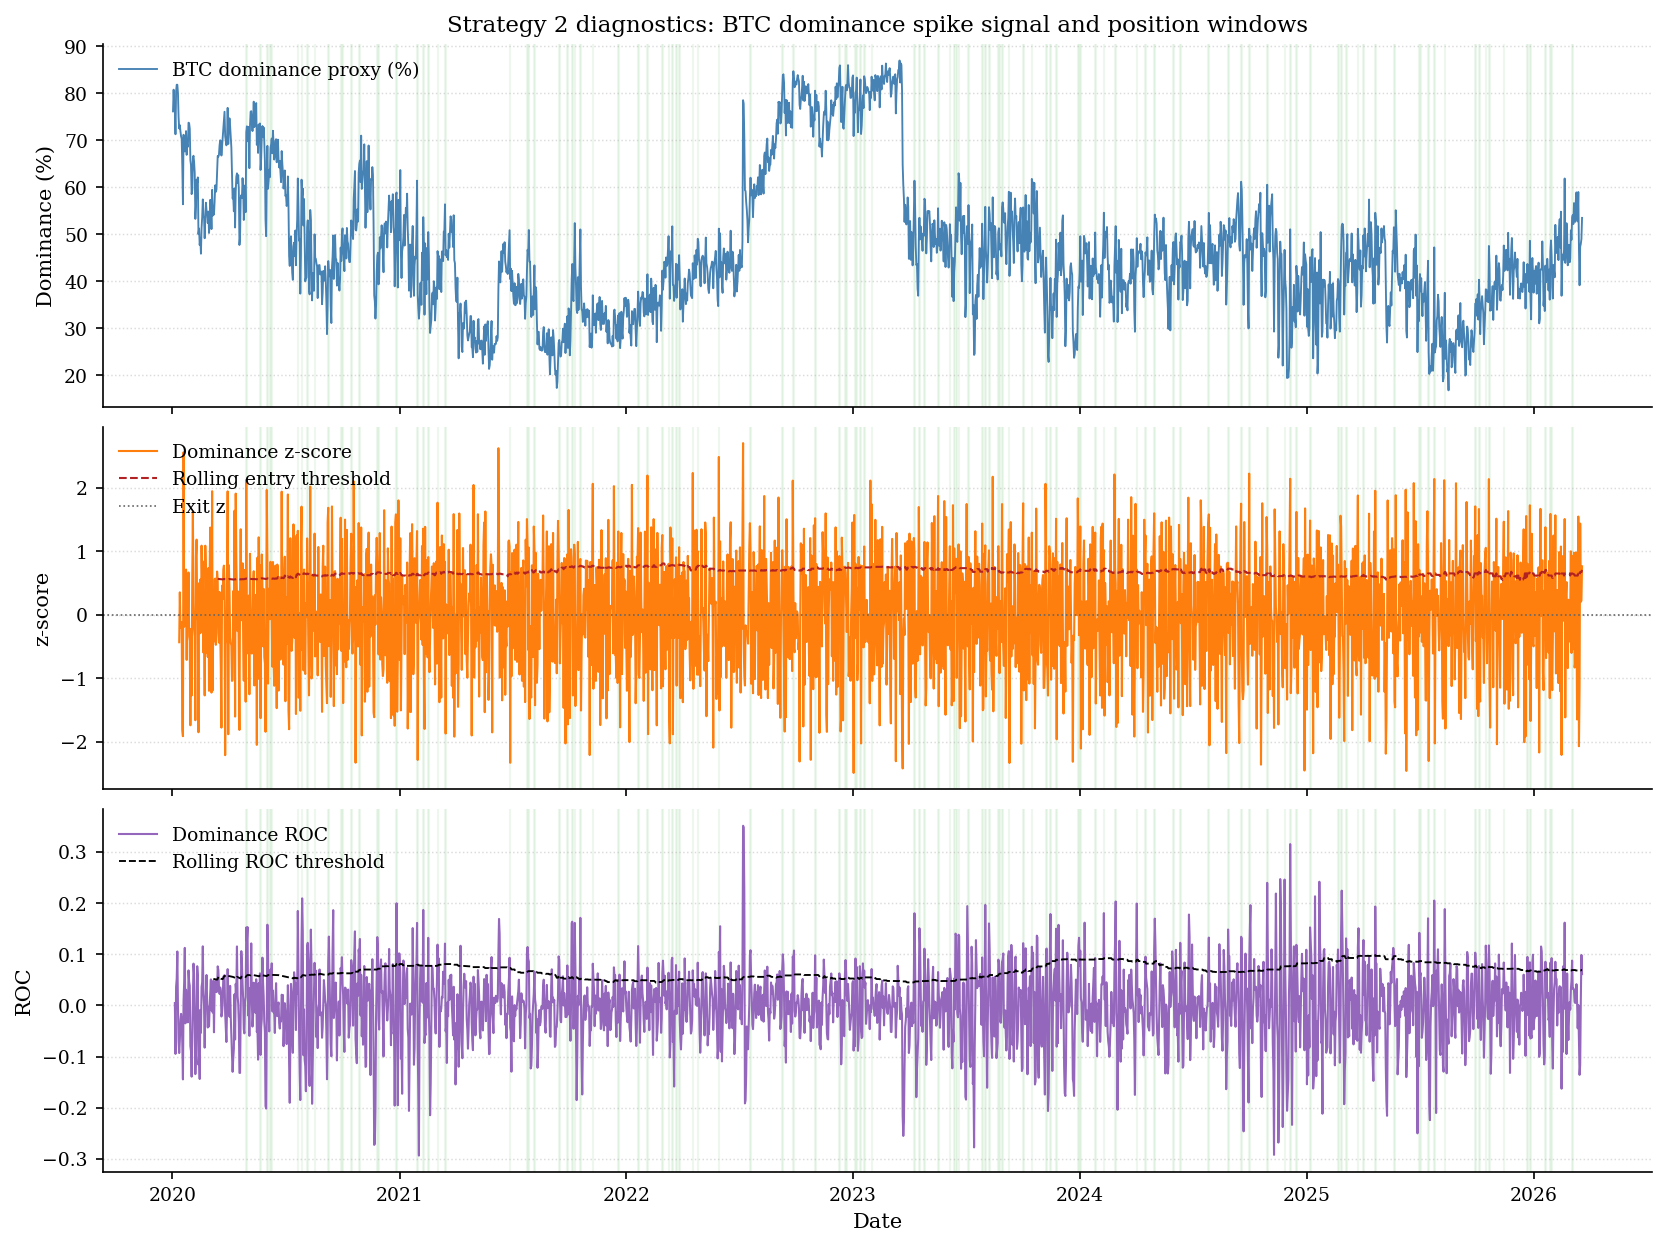
\includegraphics[width=\textwidth]{output/btc_dominance_rsi.png}
  \caption{BTC dominance ratio and RSI(14) of dominance over the full sample.  Horizontal dashed lines at RSI~$= 70$ and $30$ mark the traditional overbought/oversold thresholds.}
  \label{fig:dom-rsi}
\end{figure}


% =============================================================================
% SECTION 3 — Transaction Costs [10 points]
% =============================================================================
\section{Transaction Costs}
\label{sec:costs}

\subsection{Strategy 1: Abdi--Ranaldo Spread Estimation}

For the trend-following strategy, we adopt the Abdi and Ranaldo~\cite{abdi2017} high-low spread estimator, which exploits the full information content of OHLC bars.  The intuition is that the close price tends to lie near the bid or ask, while the midpoint of the log high and log low prices approximates the efficient price.  The estimator is:
\begin{equation}
  \hat{s}^2_t = 4 \bigl(\ln c_{t-1} - m_{t-1}\bigr)\bigl(\ln c_t - m_t\bigr),
  \label{eq:abdi-ranaldo}
\end{equation}
where $c_t$ is the close price and $m_t = (\ln h_t + \ln l_t)/2$ is the log midpoint.  We smooth via a 21-day rolling mean and compute $\hat{s}_t = \sqrt{\abs{\overline{\hat{s}^2_t}}}$.  The Abdi--Ranaldo estimator is preferred over the Roll~\cite{roll1984} model because the latter produces undefined estimates when the empirical autocovariance is positive, which occurs frequently in trending daily crypto markets.

Transaction costs are applied at each bar as:
\begin{equation}
  \text{Cost}_t = \sum_i \abs{\theta^i_t - \theta^i_{t-1}(1 + r^i_{t-1})} \times \tfrac{1}{2}\hat{s}_{t-1},
  \label{eq:cost}
\end{equation}
where $\theta^i_{t-1}(1 + r^i_{t-1})$ represents the carried (mark-to-market) position value from the previous bar, and the half-spread is lagged by one bar to prevent look-ahead bias.  The Abdi--Ranaldo estimator is already dimensionless (derived from log-price ratios), so no division by close is applied.

\subsection{Strategy 2: Flat Fee Model}

For the dominance mean-reversion strategy, we apply a flat transaction cost of 10~basis points per side on all turnover.  This is deliberately conservative relative to Binance's standard maker/taker fee schedule (which starts at 10~bps each for standard accounts and decreases with volume tiers) and subsumes both the bid-ask spread and exchange fees into a single round number.  The daily cost is:
\begin{equation}
  \text{Cost}^{S2}_t = \frac{10}{10{,}000} \sum_i \abs{w_{i,t} - w_{i,t-1}},
  \label{eq:cost-s2}
\end{equation}
where $w_{i,t}$ are the execution weights.


% =============================================================================
% SECTION 4 — Performance [10 points]
% =============================================================================
\section{Performance}
\label{sec:performance}

\subsection{PnL Construction}

We compute the total PnL series as specified in the brief:
\begin{equation}
  \Delta V_t = \sum_{i=1}^{k} \theta^i_t \, r^i_t - \text{Cost}_t,
  \label{eq:pnl}
\end{equation}
with the equity curve $V_t = V_{t-1} + \Delta V_t$ and $V_0 = \$10{,}000$.  Capital not allocated to positions is held as USDT cash and earns no return.  A circuit-breaker mechanism monitors equity at each bar and triggers full liquidation ($\theta_{i,t} = 0$ for all $i$ and all subsequent $t$) if equity reaches zero, preventing the backtest from continuing to trade through insolvency.

For Strategy~2, the portfolio value evolves multiplicatively: $V^{S2}_t = V_0 \prod_{s=1}^{t}(1 + r^{\text{net}}_{s})$, where $r^{\text{net}}_{s}$ is the daily net-of-cost portfolio return from the weighted basket.

\subsection{Reinvestment Logic}

Strategy~1 maintains a fixed gross exposure cap of $\$100{,}000$ throughout the backtest, regardless of the evolution of equity.  This design choice reflects a constant-leverage risk management philosophy: the absolute dollar exposure---and therefore the dollar-denominated risk per bar---remains bounded, while the effective leverage ratio adjusts as equity grows or shrinks.  The alternative of reinvesting profits would compound both returns and drawdowns geometrically.  Under our fixed-cap approach, the strategy's dollar PnL at any bar is bounded by $G \times \max_i \abs{r_{i,t}}$.

Strategy~2 operates with weight-based allocation and implicitly reinvests, as $V^{S2}_t$ compounds through the product of gross returns.

\subsection{Performance Metrics}

We report the following risk-adjusted performance ratios, all computed on net-of-cost returns:

\textbf{Sharpe ratio.} Annualised as $S = \sqrt{T} \times \bar{r} / \hat{\sigma}_r$, where $T = 252$ (trading days per year, the standard convention for daily data), $\bar{r}$ is the sample mean of daily returns, and $\hat{\sigma}_r$ is the sample standard deviation (with Bessel's correction, $\text{ddof} = 1$).

\textbf{Sortino ratio.} Annualised as $\text{Sortino} = \sqrt{T} \times \bar{r} / \hat{\sigma}_d$, where $\hat{\sigma}_d$ is the standard deviation of downside returns only (returns below zero, $\text{ddof} = 0$).

\textbf{Calmar ratio.} Defined as $\text{Calmar} = \text{CAGR} / \abs{\text{MDD}}$, where $\text{CAGR} = (V_T / V_0)^{T/n} - 1$ is the compound annual growth rate and MDD is the maximum drawdown.

\begin{table}[H]
  \centering
  \caption{Strategy~1 (Trend) performance metrics (net of costs).  IS = in-sample (development set, $n = 2{,}144$ days), OOS = out-of-sample (final untouched test, $n = 126$ days).  All ratios are annualised.}
  \label{tab:perf-s1}
  \begin{tabular}{lccc}
    \toprule
    Metric & Full & IS & OOS \\
    \midrule
    Sharpe Ratio            & 0.44  & 0.43  & 0.69  \\
    Sortino Ratio           & 0.57  & 0.56  & 0.94  \\
    Calmar Ratio            & 0.18  & 0.17  & 1.63  \\
    Ann.\ Return (\%)       & 9.50  & 9.23  & 15.65 \\
    Max Drawdown (\%)       & $-53.83$ & $-53.83$ & $-9.59$ \\
    Total Net PnL (\$)      & 63{,}188 & 55{,}954 & 7{,}234 \\
    Mean Holding (days)     & \multicolumn{3}{c}{21.7}  \\
    \bottomrule
  \end{tabular}
\end{table}

\begin{table}[H]
  \centering
  \caption{Strategy~2 (BTC-Dominance RSI) performance metrics (net of costs).  Same IS/OOS splits as Strategy~1.}
  \label{tab:perf-s2}
  \begin{tabular}{lccc}
    \toprule
    Metric & Full & IS & OOS \\
    \midrule
    Sharpe Ratio            & 0.45  & 0.53  & $-1.27$  \\
    Sortino Ratio           & 0.29  & 0.34  & $-0.54$  \\
    Calmar Ratio            & 0.32  & 0.39  & $-1.35$  \\
    Ann.\ Return (\%)       & 7.43  & 9.05  & $-19.31$ \\
    Max Drawdown (\%)       & $-22.97$ & $-22.97$ & $-14.27$ \\
    Total Net PnL (\$)      & 45{,}292 & 54{,}476 & $-10{,}789$ \\
    Total Trades            & 110   & 105   & 5     \\
    Win Rate (\%)           & \multicolumn{3}{c}{57.3}  \\
    \bottomrule
  \end{tabular}
\end{table}

\begin{table}[H]
  \centering
  \caption{Head-to-head comparison over the full overlapping period (2{,}270~days).}
  \label{tab:comparison}
  \begin{tabular}{lccc}
    \toprule
    Metric & Trend & Dom RSI & BTC B\&H \\
    \midrule
    Total Return (\%)      & 126.38  & 90.58   & 912.25 \\
    Ann.\ Return (\%)      & 9.50    & 7.43    & 29.32  \\
    Sharpe Ratio           & 0.44    & 0.45    & 0.76   \\
    Calmar Ratio           & 0.18    & 0.32    & 0.38   \\
    Max Drawdown (\%)      & $-53.83$ & $-22.97$ & $-76.63$ \\
    Ann.\ Volatility (\%)  & 31.96   & 19.60   & 51.30  \\
    \bottomrule
  \end{tabular}
\end{table}

Both strategies deliver positive risk-adjusted returns over the full sample, though both underperform a passive BTC buy-and-hold allocation in terms of total return.  However, both strategies achieve substantially lower maximum drawdowns than the buy-and-hold benchmark ($-53.83\%$ and $-22.97\%$ vs.\ $-76.63\%$), and Strategy~2 does so with approximately one-third of the benchmark's annualised volatility.  The rolling 60-day return correlation between the two strategies averages $0.027$, confirming that they exploit largely orthogonal sources of return: Strategy~1 captures persistent directional trends, while Strategy~2 captures short-lived mean-reversion in cross-sectional rotation.

\begin{figure}[H]
  \centering
  % 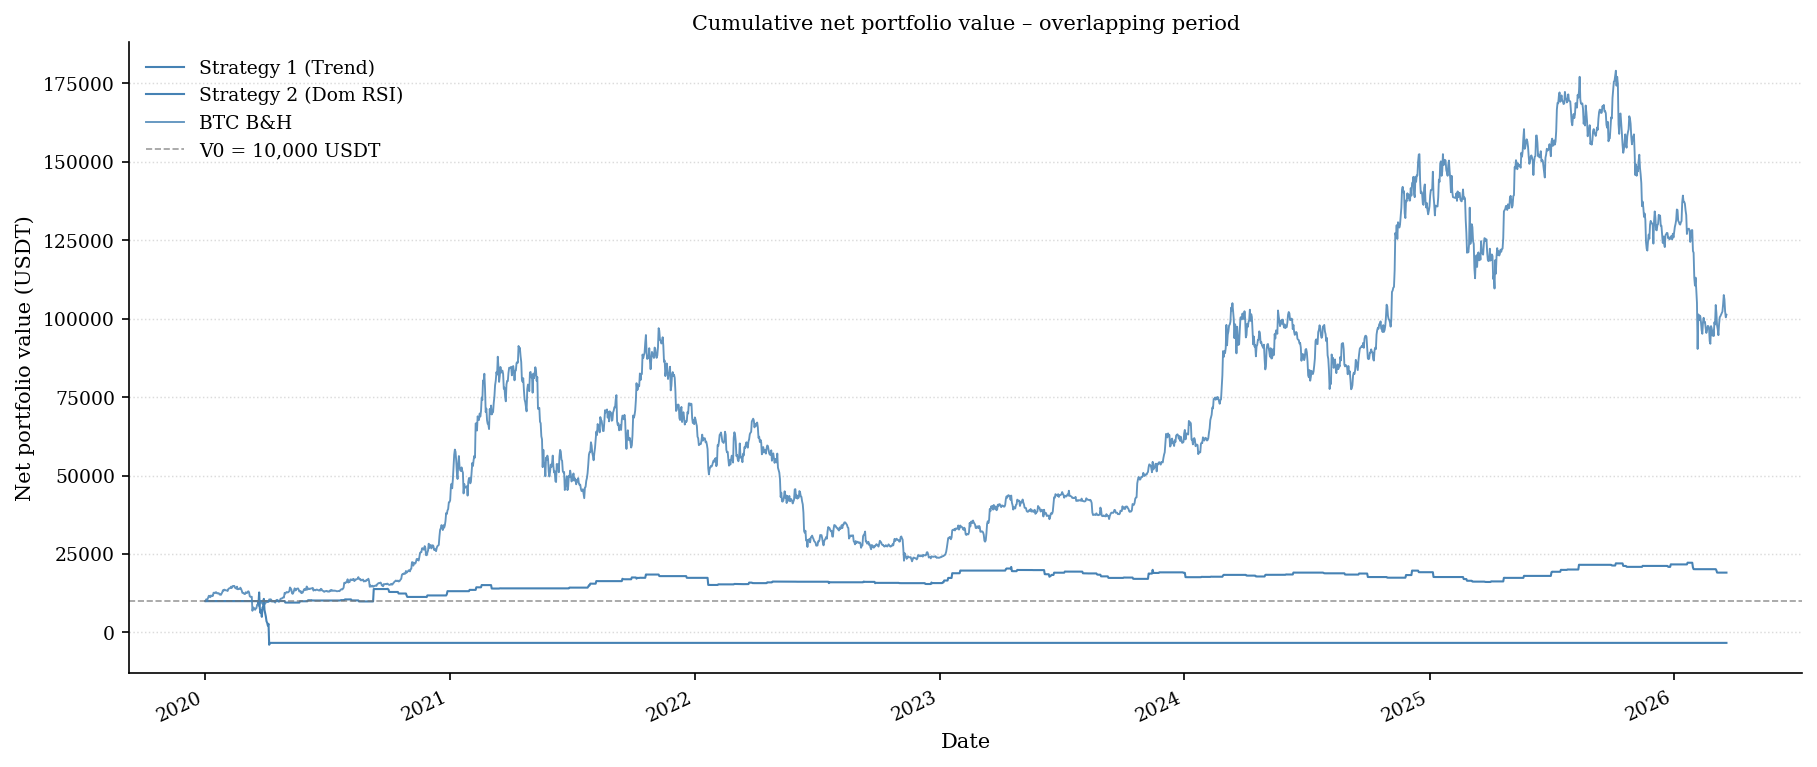
\includegraphics[width=\textwidth]{output/s2_head_to_head_wealth.png}
  \caption{Cumulative net portfolio value for both strategies and BTC buy-and-hold over the full overlapping period.}
  \label{fig:combined-equity}
\end{figure}


% =============================================================================
% SECTION 5 — Next Steps [10 points]
% =============================================================================
\section{Next Steps}
\label{sec:next-steps}

\subsection{Regime Dependence and Market Conditions}

The trend-following strategy is expected to perform well during sustained directional moves (e.g.\ the 2020--2021 bull market, the 2022 bear market) and poorly during range-bound or choppy conditions where the moving-average signal generates frequent false breakouts.  Conversely, the dominance-RSI strategy thrives in episodes of acute risk-off rotation where capital concentrates briefly into BTC before reverting, but suffers during sustained shifts in market structure (e.g.\ prolonged altcoin bear markets where the mean-reversion thesis does not apply).  The complementary nature of these two strategies provides a degree of natural diversification: the near-zero rolling correlation ($\bar{\rho} = 0.027$) confirms that periods hostile to one strategy are not systematically hostile to the other.

The Strategy~2 OOS performance (Sharpe~$= -1.27$) illustrates a key limitation: the final 126-day holdout window (November~2025 to March~2026) coincided with a BTC-dominated drawdown in which altcoins underperformed persistently, violating the mean-reversion assumption.  The tuned Optuna specification produced zero holdout trades, correctly recognising the absence of entry conditions but yielding a flat return that is uninformative for out-of-sample evaluation.  This should be reported as a quiet-regime outcome rather than a strategy failure.

\subsection{Overfitting and Robustness}

The walk-forward validation procedure mitigates but does not eliminate overfitting risk.  Strategy~1 shows encouraging IS-to-OOS stability: the Sharpe ratio actually improves from $0.43$ in-sample to $0.69$ out-of-sample, suggesting that the selected parameters generalise well to the specific holdout window.  Strategy~2 exhibits substantial degradation ($0.53 \to -1.27$, a $342\%$ decline), which is partly attributable to the regime mismatch described above and partly to the inherently episodic nature of the dominance-rotation signal (only 5 holdout trades were generated under the baseline specification, too few for statistical reliability).

The stability penalty ($\lambda = 0.1$ for Strategy~1, $0.15$ for Strategy~2) in the walk-forward scoring functions partially addresses overfitting by penalising high cross-fold variance, but cannot protect against systematic regime changes between the development and holdout periods.  The inactivity penalty in Strategy~2's scoring function ($P_{\text{inactivity}}$) further guards against parameter configurations that achieve high Sharpe by trading too rarely to be statistically meaningful.

\subsection{Proposed Improvements}

Several concrete extensions would strengthen the framework.  First, a volatility regime filter---for instance, classifying the market as ``trending'' or ``mean-reverting'' based on the Hurst exponent or the ratio of short-term to long-term realised volatility---could dynamically adjust gross utilisation or disable a strategy entirely in hostile regimes.  Second, an ensemble approach that combines trend and dominance-RSI signals with adaptive weighting (e.g.\ inverse-variance weighting based on rolling OOS performance of each strategy over the previous $N$ bars) could improve the stability of aggregate returns.  Third, the transaction cost model for Strategy~1 could be enhanced by incorporating exchange-specific maker/taker fee schedules alongside the Abdi--Ranaldo spread-based estimates, and the Strategy~2 flat-fee model could be replaced with an asset-specific spread estimator.  Fourth, the Strategy~2 basket construction could be extended to incorporate momentum or quality factors beyond the current underperformance-and-inverse-volatility tilt.  Finally, given the near-zero correlation between the two strategies, a capital-split approach allocating a fixed fraction to each strategy and rebalancing periodically would likely deliver a superior risk-return profile compared to either strategy in isolation.


% =============================================================================
% References
% =============================================================================
\bibliographystyle{plainnat}
\begin{thebibliography}{10}

\bibitem{roll1984}
R.~Roll.
\newblock A simple implicit measure of the effective bid-ask spread in an
  efficient market.
\newblock \emph{Journal of Finance}, 39(4):1127--1139, 1984.

\bibitem{abdi2017}
F.~Abdi and A.~Ranaldo.
\newblock A simple estimation of bid-ask spreads from daily close, high, and
  low prices.
\newblock \emph{Review of Financial Studies}, 30(12):4437--4480, 2017.

\bibitem{liu2021}
Y.~Liu and A.~Tsyvinski.
\newblock Risks and returns of cryptocurrency.
\newblock \emph{Review of Financial Studies}, 34(6):2689--2727, 2021.

\bibitem{moskowitz2012}
T.~J. Moskowitz, Y.~H. Ooi, and L.~H. Pedersen.
\newblock Time series momentum.
\newblock \emph{Journal of Financial Economics}, 104(2):228--250, 2012.

\bibitem{jegadeesh1993}
N.~Jegadeesh and S.~Titman.
\newblock Returns to buying winners and selling losers: Implications for stock
  market efficiency.
\newblock \emph{Journal of Finance}, 48(1):65--91, 1993.

\bibitem{engle1987}
R.~F. Engle and C.~W.~J. Granger.
\newblock Co-integration and error correction: Representation, estimation, and
  testing.
\newblock \emph{Econometrica}, 55(2):251--276, 1987.

\bibitem{bergstra2011}
J.~Bergstra, R.~Bardenet, Y.~Bengio, and B.~K{\'e}gl.
\newblock Algorithms for hyper-parameter optimization.
\newblock In \emph{Advances in Neural Information Processing Systems}, 2011.

\end{thebibliography}

\end{document}
